%
In the previous chapter only very basic linear methods for classification were discussed. The log odds were modeled in a linear fashion and a decision boundary was drawn based on this. Now the framework changes completely. The linearity assumptions are removed along with restrictions on number of classes. 
In this chapter classification trees will be discussed. They are the foundation of this report. Later, attempts to enhancing their performance will be made through different ensemble methods. 

\section{The tree}
\label{sec:Tree}
<<cartSim, echo=FALSE>>=
# Simple simulation to get nice areas and tree
source("../code/cartSim.R")
@

A classification tree makes local decisions based on a subset of the predictors. This means that the data is split in subsets, that are again split in new subsets (independently of each other) and so on. 
At the end the subsets are given a class label based on some vote-measure between the data points, usually the majority.
The voting proportions can also be used to estimate the class probabilities, if they are of interest.
An example of such a tree can be found in Figure~\ref{fig:cart}.

The simplicity of the rules make trees very general, both in terms of decision boundaries and in type of predictors. The methods usually work with continuous, discrete ordered, and categorical features. However, only continuous features will be covered in this report.  

The splits for a tree are easy to visualize, which make trees highly interpretable. Prediction is done by following splits down to the decision node, giving the predicted class. An example of such a tree can be found in Figure~\ref{fig:cartTree1}.
\\
\begin{figure}[htbp]
  \centering
  \begin{subfigure}[b]{0.48\textwidth}
    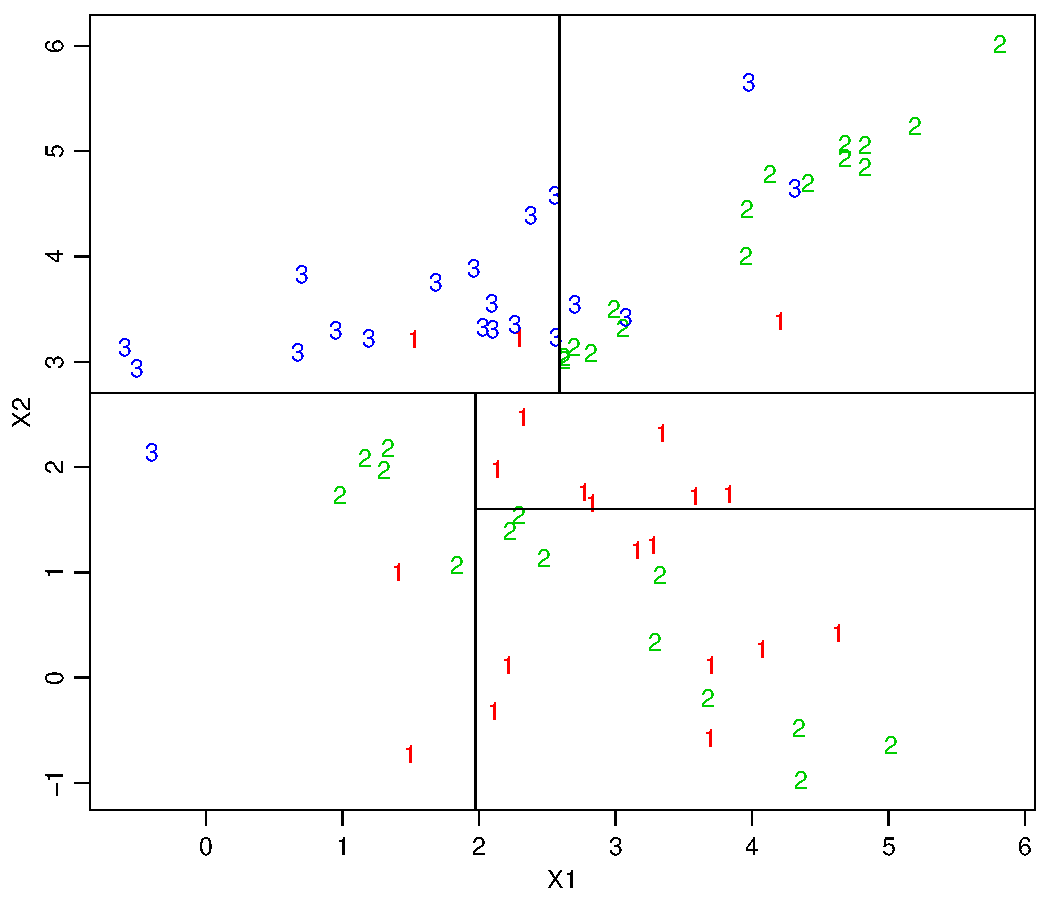
\includegraphics[width=\textwidth]{./figures/cartAreas1.pdf}
    \caption{Decisions displayed as boxes.}
    \label{fig:cartAreas1}
  \end{subfigure}%
  \quad
  \begin{subfigure}[b]{0.48\textwidth}
    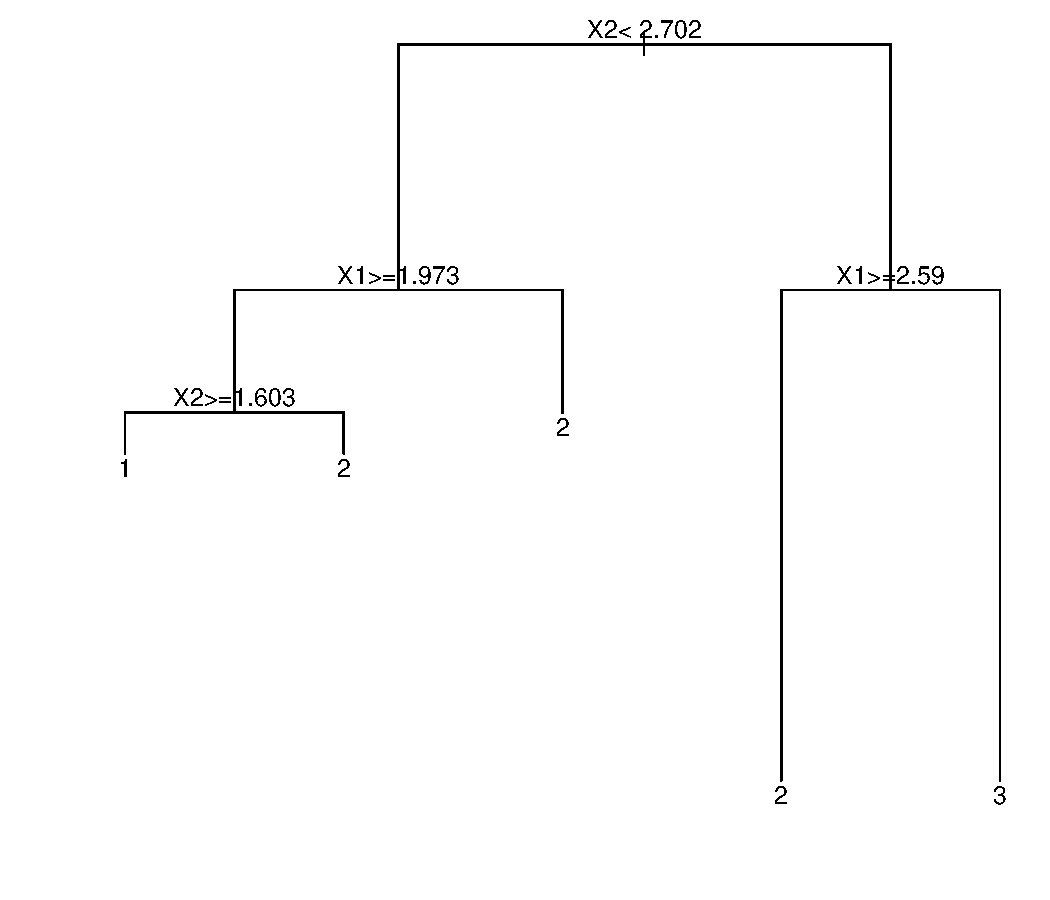
\includegraphics[width=\textwidth]{./figures/cartTree1.pdf}
    \caption{Decisions displayed as a tree.}
    \label{fig:cartTree1}
  \end{subfigure}
          %(or a blank line to force the subfigure onto a new line)
  \vspace{1\baselineskip}
  \caption{CART run on simulated data in two dimensions. }
  \label{fig:cart}
\end{figure}
\\
Unlike linear classifiers, the decision boundaries for trees can take many different forms. Everything from a linear boundary with two end nodes, to a highly complex boundary with the same amount of end nodes as data points, is possible. In this regard, the terms \textit{overfitting} and \textit{underfitting} need to be introduced. 

An underfitted model is too simple to capture the complexity of the data. On the contrary, an overfitted model is fitted to close to the training data and as a result describes the random noise of the training data rather than the true underlying model.  Obviously, a full tree, i.e. only one training point in each end node, will be overfitted, while a too small thee will be underfitted. 

In the regression framework, under squared error loss, it can be shown that a small tree is highly biased with low variance, while a larger tree is highly unstable (high variance), but with smaller bias. 
In appendix~\ref{sub:Bias-variance tradeoff}, it is shown how the $\mathrm{EPE}$, introduced in \ref{sub:LDA}, has an additive relationship with the classifier's bias and variance. As a result, the \textit{bias-variance tradeoff} should be considered when creating the prediction method. 

For classification the same argument does not quite hold, but similar definitions for bias and variance has been proposed for $0/1$ loss in the literature. Some of the most well known methods include \cite{kong1995error}, \cite{kohavi1996bias}, \cite{breiman1996bias} and \cite{Friedman1997bias}. While they have all provided useful insight to classification problems, non of them present a framework as simple and satisfactory as for regression. In this report, when referring to bias or variance of classifiers, it is more in a heuristic way. Loosely, bias measures the systematic error of a classifier, i.e. the average error over different training sets. Variance measures the additional error do to variations in the classifier between training sets. 
\\
\\
There are proposed different algorithms for building classification trees. They all try to find the optimal balance between bias and variance. This is done in terms of how the tree is grown, but more importantly, how to control the size of the tree. 
Some of the more common methods include ID3 by \cite{ID3}, C4.5 by \cite{C4.5} and its successor See5/C5.0, CHAID by \cite{CHAID} and CART by \cite{breiman}.
In this report only CART will be covered, as it is one of the more widely used.
%
\section{CART}
\label{sec:CART}
%
The Classification and Regression Trees algorithm split at only \textit{one} variable at a time, i.e. no combinations of features are used in the splits. This means that the domain is split into rectangles, aligned with the axes. 
Also, each split in CART divide the domain in \textit{two} parts, often referred to as binary splitting. Thus, the splits are done in the simplest way possible. Nevertheless, CART has shown decent performance. 

CART, as the name implies, can be used both for classification and regression, but only its abilities as a classifier will be considered in this section. The regression framework will be briefly introduced in \ref{sec:Gradient Boosting}.
\\
\\
In Figure~\ref{fig:cart} a toy example was simulated to illustrate how the CART algorithm works. The tree is made by the R function \verb+rpart+ by \cite{rpart}. To make it easy to visualize, only two predictors were used. 
In Figure~\ref{fig:cartAreas1} the domains resulting by the splits are displayed. Each vertical and horizontal line shows a split. It is clear that the data is not linear, and the figure shows how the algorithm is capable of handling such a complex decision boundary.
For more than two predictors it is hard to visualize the splits on the actual domain, so a tree view is used instead.
 In Figure~\ref{fig:cartTree1} the tree from the toy example is displayed. It is clear that it easily generalizes to more than two dimensions. \\
%
\subsection{Growing a tree}
\label{sub:Growing a tree}
The intuition behind CART is quite simple. Now, the splitting decisions need to be investigated. As it is too computationally expensive to create an optimal tree based on the training data, greedy algorithms for splitting in a sequential matter are used instead. A split needs to to be based on a criterion and one of the more common is the \textit{Gini index}. For $K$ classes it is defined as,
\begin{align}
  Q_m(T) &= \sum^{K}_{k=1} \hat{p}_{mk} (1 - \hat{p}_{mk}),  \\ 
  \label{eq:pmk} 
  \text{where}& \quad \hat{p}_{mk} = \frac{1}{N_m} \sum_{\mathbf{x}_i \in R_m} I\{y_i = k\}.
\end{align}
Here $T$ is the tree, $m$ is a node, $N_m$ is the number of data points in node $m$, $y_i$ is the class of training point $i$ and $R_m$ is the region defined by the node.
$\hat{p}_{mk}$ is therefore the proportion of class $k$ in node $m$.
The Gini index increase with the diversity in the node, and gives therefore a measure of \textit{node impurity}. For nodes with only one class it is zero, and for homogeneous nodes (equal amounts of all classes) it gets its maximum value. The greedy step done in CART finds the split that gives the lowest total node impurity, and weight the two nodes by their size.  
The length of the branches in Figure~\ref{fig:cartTree1} is a representation of the reduction in node impurity. The longer the branch the higher the gain.

Now, consider the case where a split is performed on node $P$. By splitting on the variable $x_j$, let $R_L(j,s) = \{\mathbf{x} | x_j \leq s\}$ denote the region of the "left" split,  and $R_R(j,s) = \{\mathbf{x} | x_j > s\}$ denote the "right". The solution to which variable $x_j$ and split point $s$ that gives the lowest node impurity can then be found by,
\begin{align}
  \{x_j^*, s^*\} = \argmin_{x_j,s} \left\{ \frac{N_L}{N_P} Q_L(T)
  + \frac{N_R}{N_P} Q_R(T) \right\}.
\end{align}
Here $x_j$ and $s$ lies in $\hat{p}_{mk}$ in \eqref{eq:pmk}. $N_L$, $N_R$ and $N_P$ are the number of observations in the left, right and parent node respectively.
\\
\\
There are other similar measures of node impurity, like \textit{deviance} and \textit{misclassification error}. Deviance is defined as,
\begin{align}
  Q_m(T) = -  \sum^{K}_{k=1} \hat p_{m k} \log \hat p_{m k},
\end{align}
and misclassification error as,
\begin{align}
  \label{eq:CARTmisclass} 
  &Q_m(T) = \frac{1}{N_m} \sum_{\mathbf{x}_i \in R_m} I\{y_i \neq k^*\} = 1 - \hat p_{m k^*},\\
  &\text{where} \quad k^* = \argmax_k \hat p_{m k}. \notag
\end{align}
Unlike the Gini index and the deviance, the misclassification error is not differentiable. This makes it hard to use for numerical optimization, so Gini or deviance are usually the preferred choice. 

\subsection{Pruning}
\label{sub:Pruning}

When creating a tree it is important to consider the tree size. One simple way to restrict the tree size would be to stop when the total node impurity change less than some threshold. This does not take into account that a seemingly worthless split might cause an excellent successive split. 
What CART does instead is to grow a large tree and then \textit{prune} it back to find a local optimum. Here pruning refers to collapsing some number of internal nodes in the tree. 

Let $T_0$ denote the full tree and $T$ a subtree of $T_0$ that can be obtained by pruning. $|T|$ is the number of terminal nodes and $R_{\tau}$ is the region of the terminal node $\tau$. The goal is to find the subtree $T_\alpha$ that minimizes some cost function $C_\alpha (T)$, usually the total terminal node impurity, but regularized by penalizing on the number of terminal nodes,
\begin{align}
  \label{eq:CostPruning} 
  C_\alpha (T) = \sum_{\tau = 1}^{|T|} Q_\tau (T) + \alpha |T|. 
\end{align}
This method is referred to as \textit{cost-complexity pruning}.
Here both the Gini index and deviance can be used for $Q_\tau (T)$, but it might be more common to use the misclassification rate in \eqref{eq:CARTmisclass}. Probably because the actual objective is to minimize the expected prediction error under 0/1 loss.

The optimization problem in \eqref{eq:CostPruning} mights seem hard to solve. However, \cite{breiman} suggested a method called \textit{weakest link} pruning to find $T_\alpha$. The idea is to sequentially collapse the nodes that gives the smallest increase in $C_\alpha(T)$.
They proved that if continuing to collapse all the way back to a single node, $T_\alpha$ has to be in this sequence of subtrees. It is usually not that high a cost to prune back to the root node, so it is a commonly used method.

The choice of $\alpha$ is also important to consider. This is usually done through cross-validation, or, if the dataset is large, through test error on a separate set not used to build the tree. The latter is less computationally expensive, but can only be used on larger datasets. 
The final tree chosen is not necessarily the tree with the lowest misclassification error. Another common practice is to use the most parsimonious tree within one standard deviation of the minimum.


